\chapter{Les missions effectuées}
\label{chap:Chapter 4 title}
\section*{Introduction}

\hspace{16pt}Ce chapitre est consacré à la description des missions effectuées durant le stage. Chaque mission représente une étape clé dans le développement du chatbot, depuis la configuration initiale jusqu'à la mise en ligne. Nous aborderons la configuration des environnements de développement, la création et la gestion des bases de données, et le développement des interfaces utilisateur. En détaillant ces missions, nous mettrons en lumière les compétences techniques mobilisées et les défis rencontrés. Ce chapitre vise à illustrer le processus de développement et les contributions spécifiques apportées à chaque étape du projet.

\pagebreak

\section{Le Chatbot}

\subsection{Configuration static}

\hspace{16pt}La configuration statique du chatbot concerne les éléments du chatbot qui sont définis à l'avance et qui ne changent pas dynamiquement en fonction des interactions utilisateur. Voici quelques aspects clés de cette configuration:

\begin{itemize}
  \item \textbf{Réponses prédéfinies: }Le chatbot est programmé avec une série de réponses prédéfinies pour les questions fréquentes.
  \item \textbf{Flow du prise de rendez-vous: }Définir un flux statique qui accompagnera l'utilisateur dans sa prise de rendez-vous.
  \item \textbf{Interface utilisateur: }La présentation et les options initiales du chatbot, telles que les boutons de démarrage et les messages de bienvenue, sont configurées statiquement.
  \item \textbf{Connexion: }Configurer un processus statique permettant aux utilisateurs de se connecter avant d'utiliser certaines fonctionnalités du chatbot.
  \item \textbf{Inscription: }Mettre en place un processus d'inscription statique pour les nouveaux utilisateurs, leur permettant de créer un compte avant d'accéder aux fonctionnalités du chatbot.
\end{itemize}

\begin{figure}[H] 
    \centering
    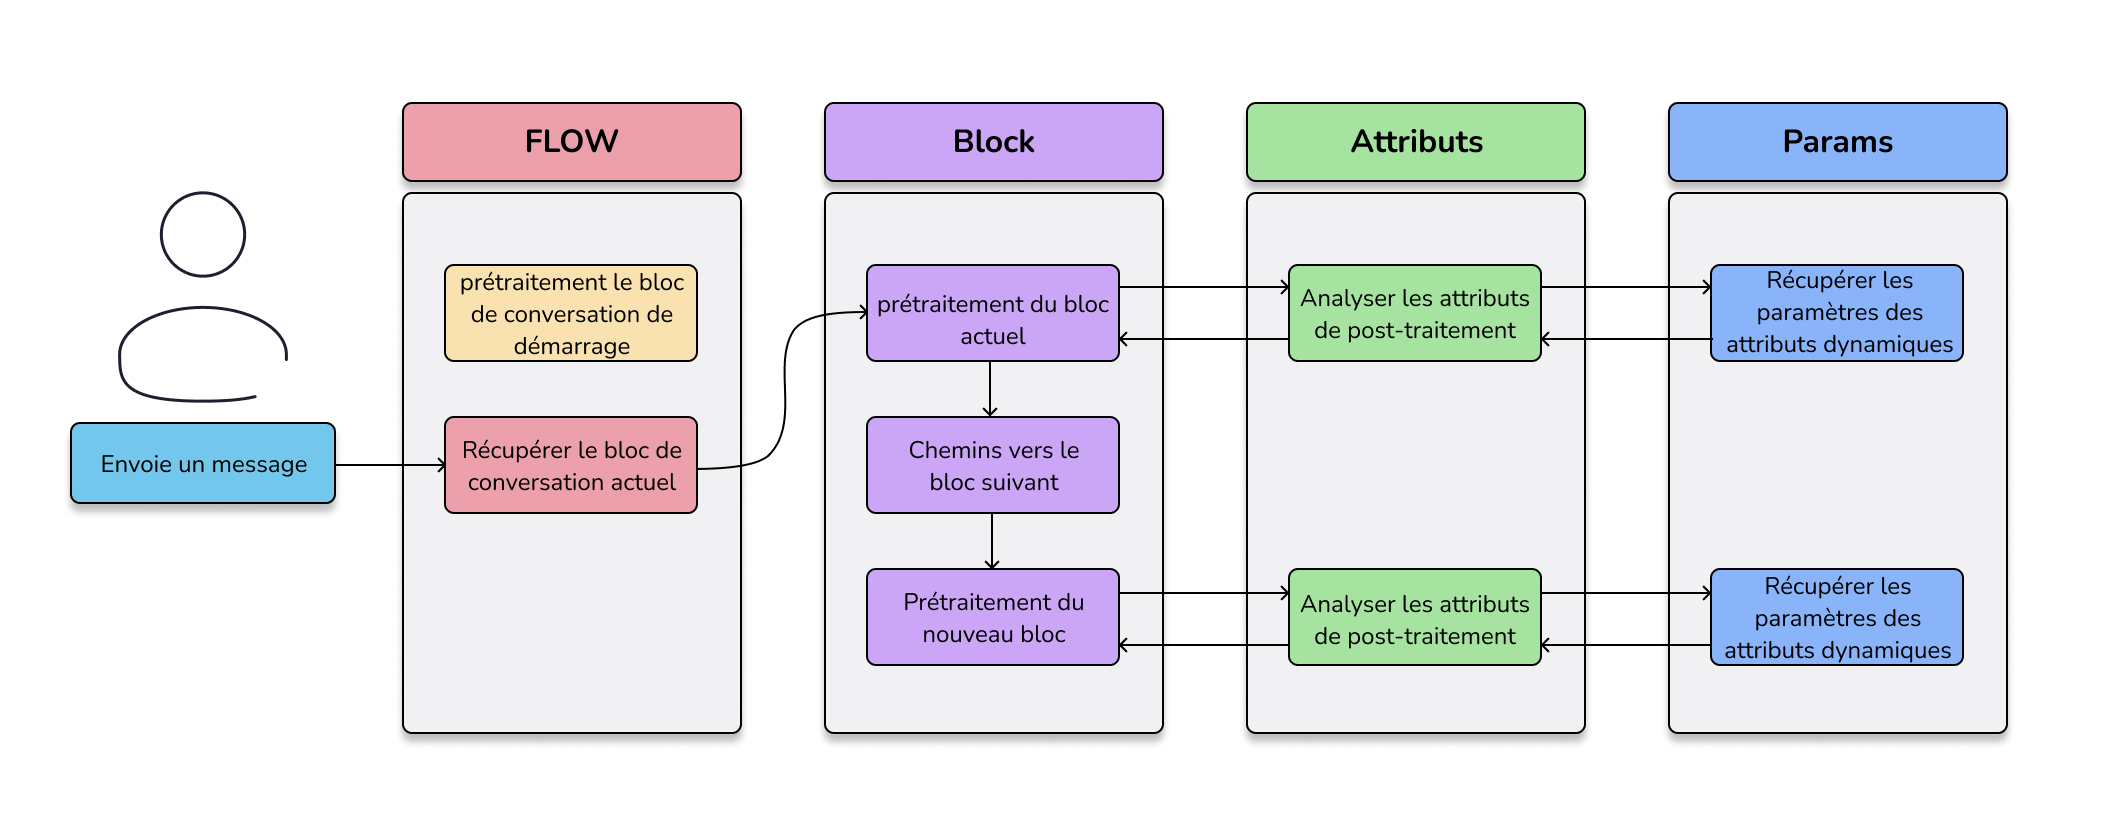
\includegraphics[scale=0.5]{Figures/chatbot.png}
    \caption{Structure générale du configuration Chatbot}
\end{figure}

\subsection{Configuration dynamique}

\hspace{16pt}Concernant les aspects dynamiques de notre chatbot, il nous a été demandé de le rendre « entièrement » personnalisable, ce qui signifie:

\begin{itemize}
  \item \textbf{Construction dynamique: }Chaque message à l'écran doit être configurable via un tableau de bord, y compris les messages d'erreur.
  \item \textbf{Messages dynamiques: }Les messages doivent être modifiés en fonction du contexte.
  \item \textbf{Flux dynamique: }L'utilisateur doit avoir la possibilité de choisir entre où aller ensuite à partir de sa position actuelle (à l'exclusion bien sûr des flux dans lesquels nous demandons des informations critiques pour créer le compte de l'utilisateur)
  \item \textbf{Composant dynamique: }Les composants personnalisés doivent s'adapter aux entrées de l'utili-sateur et afficher les informations en conséquence.
  \item \textbf{Données dynamiques: }chaque information contenue par le chatbot provient de l'API qui connecte notre chatbot à la base de données.
\end{itemize}


\begin{figure}[H] 
    \centering
    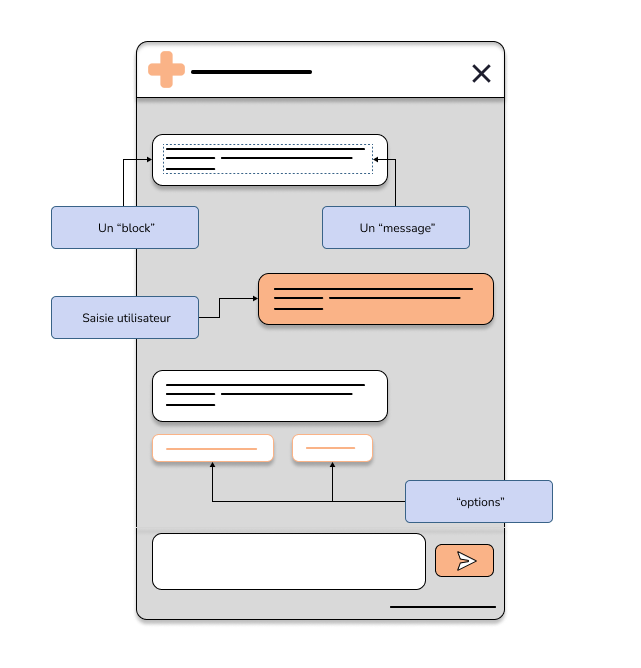
\includegraphics[scale=0.5]{Figures/cbs_general.png}
    \caption{Structure générale du Chatbot}
\end{figure}


\begin{figure}[H] 
    \centering
    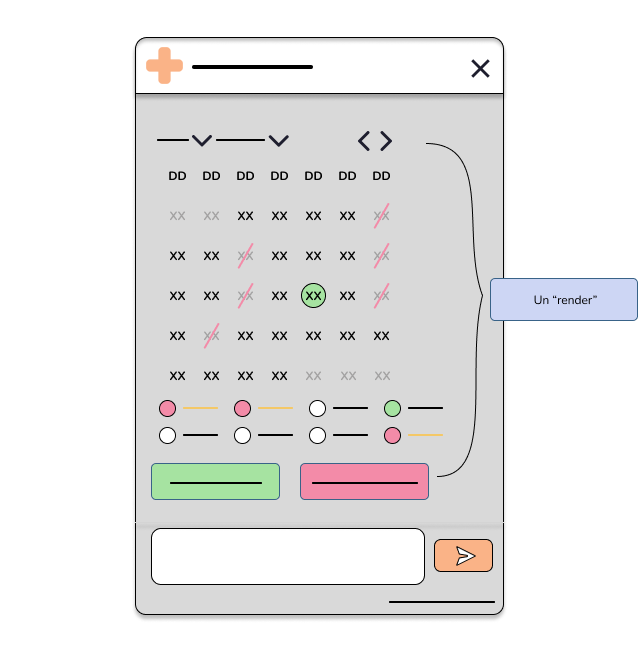
\includegraphics[scale=0.5]{Figures/cbs_render.png}
    \caption{Structure générale du Chatbot (exemple de "render" element)}
\end{figure}

\section{La base de donnéés}


\subsection{Création des entités}

\hspace{16pt}La création des entité (Figure \ref{entite}) dans la base de données est une étape cruciale pour structurer les informations de manière efficace et logique.

En structurant ces entités de manière logique et efficace, nous avons pu créer une base de données robuste et évolutive, capable de gérer les différentes facettes du projet, y compris la gestion des utilisateurs, des médecins, des rendez-vous, et des interactions du chatbot.

\subsection{Configuration d'API}

\hspace{16pt}Une API (Application Programming Interface) est un ensemble de règles permettant à des applications de communiquer entre elles. Elle utilise des protocoles comme HTTP/HTTPS pour échanger des données et donne accès à certaines fonctionnalités ou informations d'un service.

\begin{figure}[H] 
    \centering
    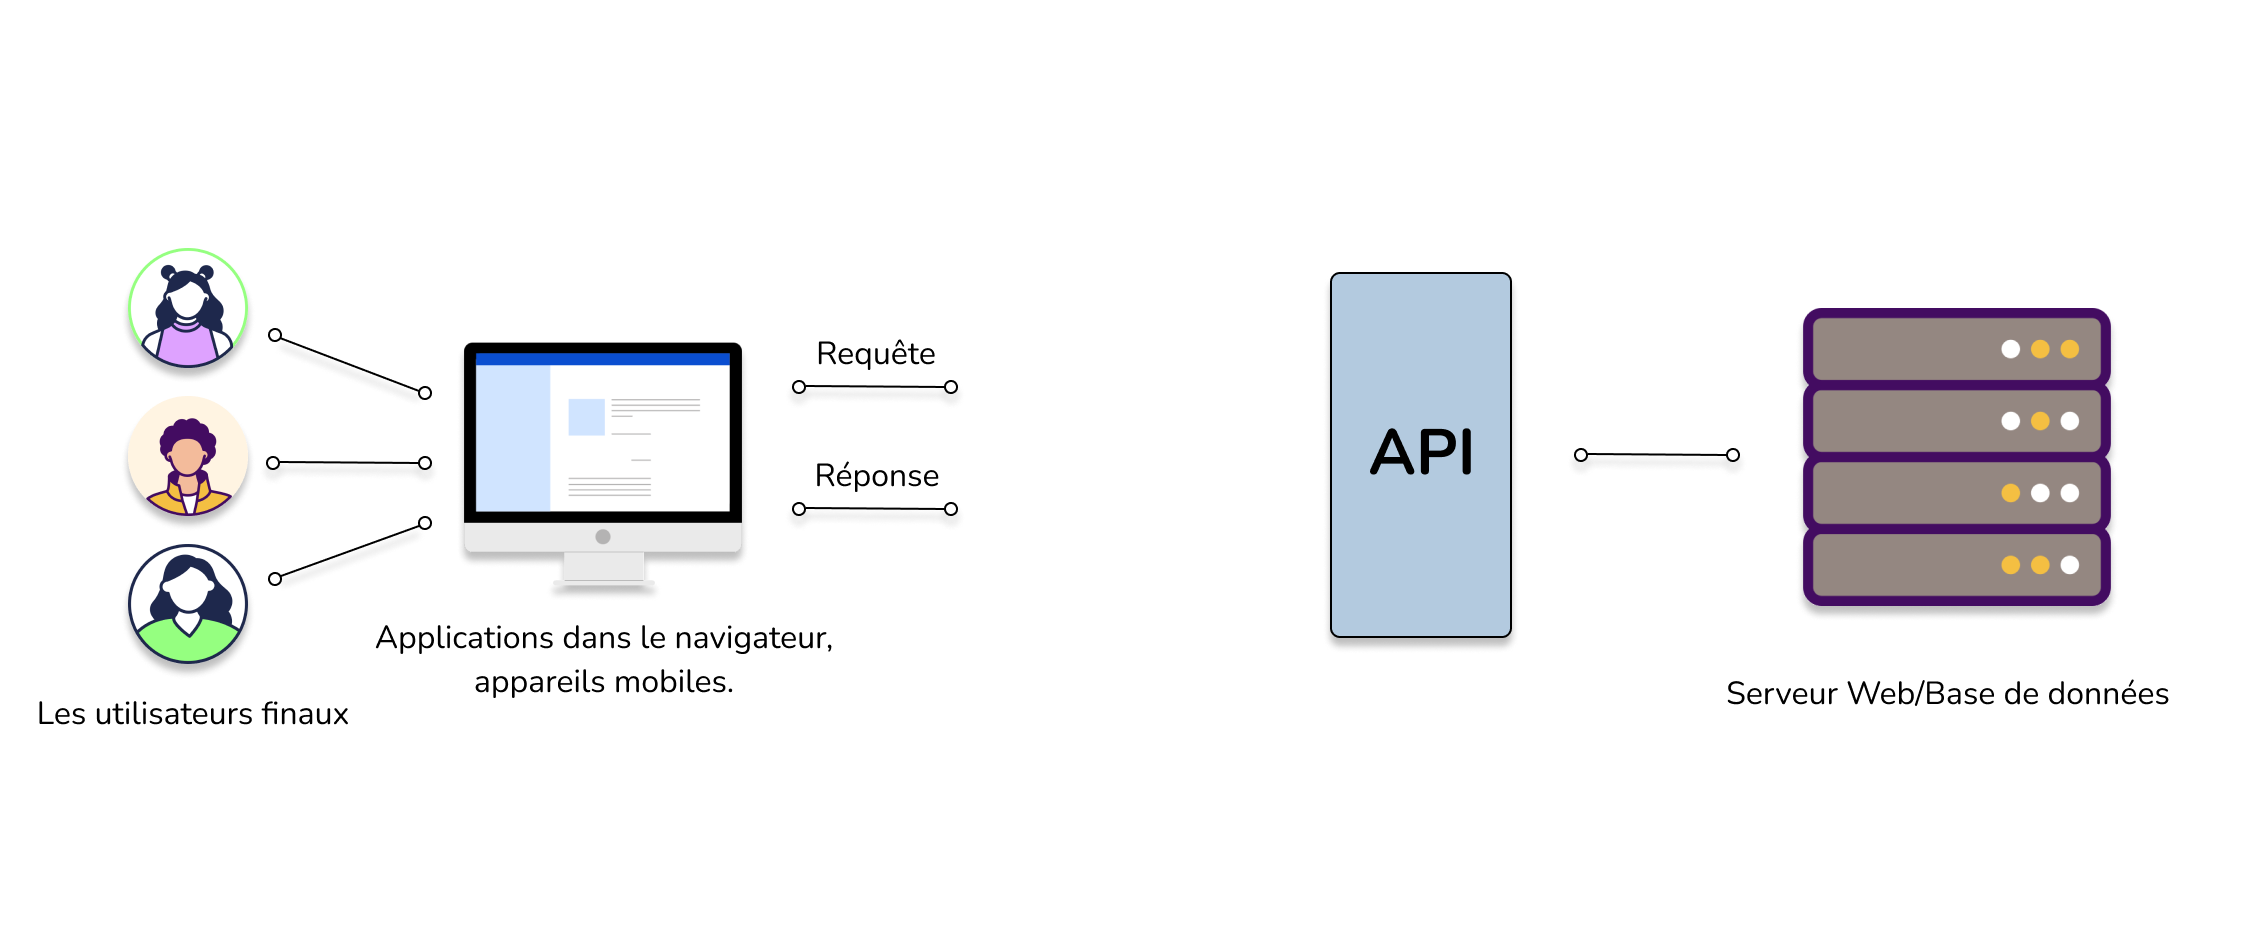
\includegraphics[scale=0.49]{Figures/API.png}
    \caption{Foncionnement d'un API}
\end{figure}

La configuration de l'API est une étape essentielle pour permettre une communication efficace entre le frontend et le backend de notre application.

Pour ce projet, nous avons utilisé Symfony avec API Platform pour créer une API RESTful. API Platform offre une grande flexibilité et permet de configurer facilement les opérations CRUD (Create, Read, Update, Delete), la validation des champs, la gestion des relations, les filtres et les groupes de sérialisation. Voici un aperçu de ces fonctionnalités:

\begin{itemize}
  \item \textbf{Opérations CRUD Configurables: }API Platform facilite la configuration des opérations CRUD pour chaque entité. Par défaut, les opérations GET, POST, PUT, DELETE sont disponibles, mais elles peuvent être personnalisées ou restreintes selon les besoins.
  \item \textbf{Validation des Champs: }API Platform intègre le composant de validation de Symfony, ce qui permet de définir des règles de validation directement dans les entités.
  \item \textbf{La gestion des relations entre les entités est simplifiée avec API Platform. Les relations peuvent être configurées pour être exposées via l'API.}
  \item \textbf{API Platform permet d'ajouter facilement des filtres pour les opérations GET. Ces filtres permettent de rechercher et de trier les données de manière flexible.}
  \item \textbf{Groupes de Sérialisation: }Les groupes de sérialisation permettent de contrôler les données qui sont exposées via l'API. Cela est utile pour restreindre les champs visibles selon le contexte (lecture, écriture, etc.).
\end{itemize}

\begin{figure}[H] 
    \centering
    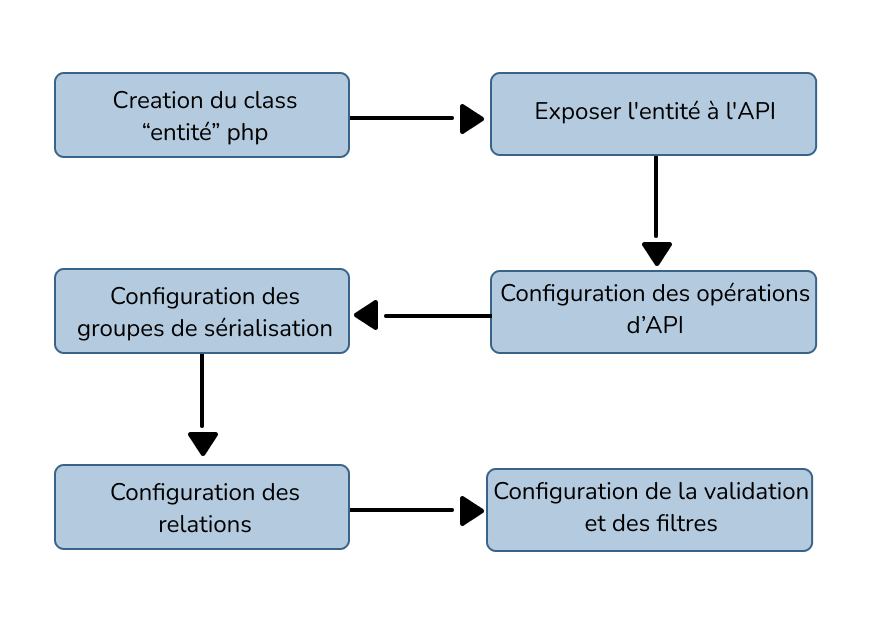
\includegraphics[scale=0.9]{Figures/api_entity.png}
    \caption{Flux général de création d'une entité API}
\end{figure}

\section{Tableau de bord}

\subsection{La gestion des rendez-vous}

\hspace {16pt}La gestion des rendez-vous est une fonctionnalité essentielle du dashboard, permettant aux admini-strateurs et aux médecins de suivre et de gérer efficacement les consultations des patients. Voici les principales caractéristiques de cette fonctionnalité:

\begin{itemize}
  \item \textbf{Vue Calendrier: }Une interface calendrier permet de visualiser les rendez-vous par jour, semaine ou mois. Les rendez-vous sont colorés en fonction de leur statut (confirmé, en attente, annulé).
  \item \textbf{Confirmation et Modification: }Les administrateurs peuvent confirmer, modifier ou annuler des rendez-vous directement depuis le dashboard.
\end{itemize}

\subsection{La gestion d'équipe medicale}

\hspace{16pt} La gestion de l’équipe médicale est une autre fonctionnalité clé du dashboard, assurant une organi-sation optimale des ressources humaines et des services offerts. Voici comment cette fonctionnalité est mise en œuvre:

\begin{itemize}
  \item \textbf{Liste des Médecins: }Une liste détaillée des médecins avec leurs spécialités, disponibilités et coordonnées. Les administrateurs peuvent facilement ajouter, modifier ou désactiver des médecins.
  \item \textbf{Planification des Horaires: }Un module de planification permet de définir les horaires de travail des médecins.
  \item \textbf{Gestion des Spécialités: }Les administrateurs peuvent gérer les spécialités médicales, en ajoutant ou supprimant des spécialités et en assignant des médecins aux différentes spécialités.
  \item \textbf{Rapports et Statistiques: }Des rapports détaillés sur les activités des médecins, incluant le nombre de consultations, le taux de satisfaction des patients, et les performances par spécialité.
\end{itemize}

\subsection{La gestion du Chatbot}

\hspace{16pt} La gestion du chatbot depuis le dashboard permet de maintenir et d’améliorer en continu l’interaction avec les patients. Voici les fonctionnalités principales de cette section:

\begin{itemize}
  \item \textbf{Configuration des F.A.Q: }Les administrateurs peuvent ajouter ou modifier les réponses pré-définies du chatbot pour les questions fréquentes. Cela inclut la mise à jour des informations sur les horaires, les services et les procédures.
  \item \textbf{Personnalisation: }Des options de personnalisation permettent de modifier le comportement du chatbot, incluant les messages de bienvenue.
\end{itemize}

\newpage

\section*{Conclusion}

\hspace{16pt}En conclusion, les missions effectuées ont permis de mettre en pratique une large gamme de compé-tences techniques et organisationnelles. Chaque étape du projet a été l'occasion d'apprendre et de s'adapter, démontrant la complexité et la richesse du processus de développement. Les compétences acquises et les défis surmontés ont non seulement contribué à la réussite du projet, mais ont également enrichi notre expérience professionnelle de manière significative.

\pagebreak
